\section{Data Comparison}
\label{sec:data_comparison}
Different comparison methods was used for data comparison. Looking on the graph representation of the data, we can see a visual similarity of the graphs. \Cref{fig:visual_IMU_similarity_example} shows an example of two independent graphs of the orientation x-element data of the same gesture. Similarity of graphs can be determined by method such as Dynamic Time Wrapping and Cross-Correlation, which is described in \cref{subsec:dtw} and \ref{subsec:cross_correlation}. 

\begin{figure}[!ht]
    \centering
    \begin{subfigure}{.5\textwidth}
        \centering
        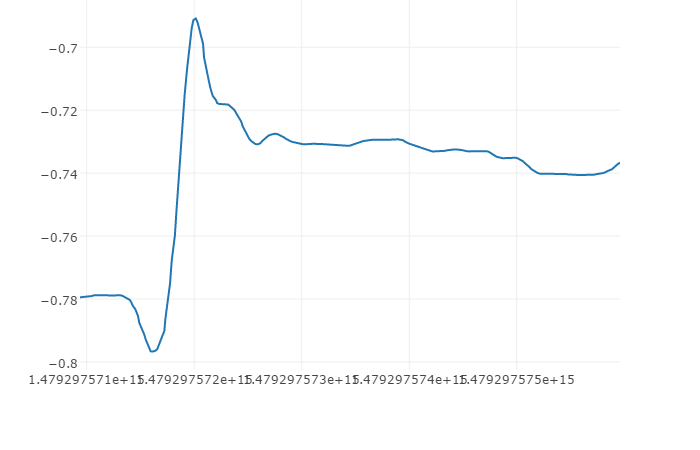
\includegraphics[height=4.5cm]{content/05-Methodology/images/eat-ori-x1.png}
        \caption{}
        \label{fig:eat_ori_x1}
    \end{subfigure}%
    \begin{subfigure}{.5\textwidth}
        \centering
        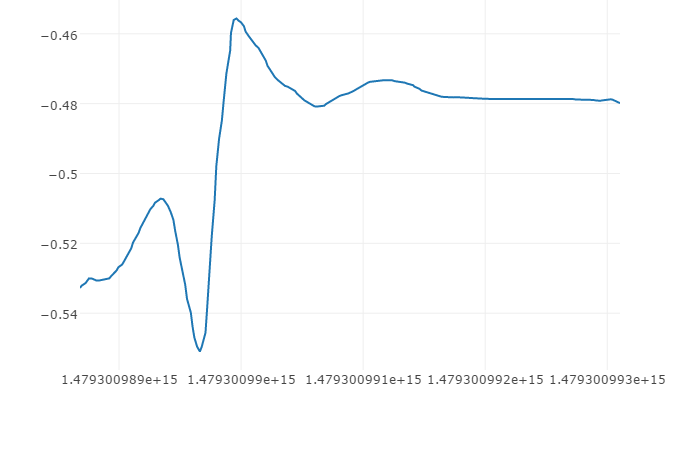
\includegraphics[height=4.5cm]{content/05-Methodology/images/eat-ori-x2.png}
        \caption{}
        \label{fig:eat_ori_x2}
    \end{subfigure}
    \caption[Visual similarity of two IMU-graphs]{The two graphs \subref{fig:eat_ori_x1} and \subref{fig:eat_ori_x2} are two independent graphs of the orientation x-element data of the same gesture. We can see some characteristics that are similar, especially where the graph is increasing and decreasing.}
    \label{fig:visual_IMU_similarity_example}
\end{figure}

Graphs from the EMG data do have similar characteristic as seen in \Cref{fig:visual_EMG_similarity_example}, but the graphs are too noisy to give a good result for comparison methods such as DTW and cross correlation. However, with some data processing we can allow the system to use DTW and cross correlation to analyse the graphs, more details on this is described in \cref{subsec:emg_analysis}.  
\begin{figure}[!ht]
    \centering
    \begin{subfigure}{.5\textwidth}
        \centering
        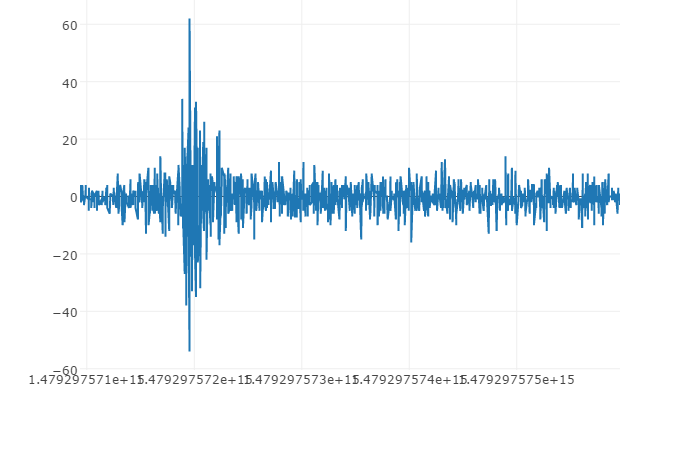
\includegraphics[height=4.5cm]{content/05-Methodology/images/eat-emg8-1.png}
        \caption{}
        \label{fig:eat_emg8_1}
    \end{subfigure}%
    \begin{subfigure}{.5\textwidth}
        \centering
        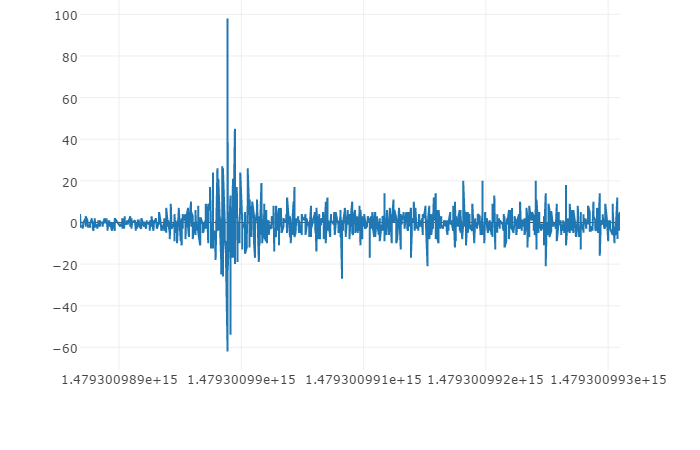
\includegraphics[height=4.5cm]{content/05-Methodology/images/eat-emg8-2.png}
        \caption{}
        \label{fig:eat_emg8_2}
    \end{subfigure}
    \caption[Visual similarity of two EMG-graphs]{The two graphs \subref{fig:eat_emg8_1} and \subref{fig:eat_emg8_2} are two independent graphs of the EMG data from the same pad of the same gesture. We can see similarity of this graphs, but unlike \cref{fig:visual_IMU_similarity_example} there is a lot of noises.}
    \label{fig:visual_EMG_similarity_example}
\end{figure}

\subsection{Dynamic Time Wrapping}
\label{subsec:dtw}
Dynamic time warping (DTW) is a well-known technique to find an optimal alignment between two given (time-dependent) sequences $x$ and $y$ under certain restrictions \cite{muller2007dynamic}. The goal is to align two sequence of graph by warping the time axis iteratively until an optimal match between the two graph is found.

DTW algorithm work with that it tries to fill a cost matrix. Each element of the cost matrix $C$ is the distance of the corresponding elements of the two sequences. Calculating C have a complexity of $\mathcal{O}(n^2)$ where $n$ and $m$ is the size of $x$ and $y$. We can define initial values of C as
\begin{align*}
    C_{0,0} &= D(x_{0},y_{0})  \\
    C_{i,0} &= C_{i-1,0} + D(x_{i},y_{0}) \\
    C_{0,j} &= C_{0,j-1} + D(x_{0},y_{j}) \\
\end{align*}
 and use this to calculate C, such that
\begin{align*}
    C_{i,j} &= min(C_{i - 1,j}, C_{i,j - 1}, C_{i - 1,j - 1}) + D(x_{i}, y_{j}) \\
\end{align*}
where $D(x_{i},y_{j})$ is the euclidean distance between the points $x_{i}$ and $y_{j}$, defined as
\begin{equation*}
    D(x_{i},y_{j}) = \sqrt{(x_{i}-y_{j})^2}
\end{equation*}
The function to calculate Dynamic Time Warping Distance returns $C_{n,m}$, in other word the last element of the matrix.

The similarity of an input to a gesture is calculated by
\begin{equation*}
    d_{g} = \sum_{s}\sum_{i}(\mean{d}_{g,i,s})
\end{equation*}
where $d_{g}$ is the distance value to gesture $g$, and $\mean{d}_{g,i,s}$ is the average distance value given from sensor $s$ of the input to an instance $i$ of the training data sets of gesture $g$. Normalized value $\hat{d}_{g}$ is given by
\begin{equation*}
    \hat{d}_{g} = 1 - \frac{d_{g}}{d_{max}}
\end{equation*}


\subsection{Cross Correlation}
\label{subsec:cross_correlation}
Cross Correlation is a method to estimate the degree of similarity of two series. Cross correlation works on any number of dimension, but for the purpose of this project, we only need to take a look at the one-dimensional cross correlation. Let $x$ and $y$ be two series, then we can define the one-dimensional normalized cross correlation $r$ at delay $d$ as	

\begin{equation}
\label{eq:cross_correlation}
    r(d) = \frac{\sum\limits_{i=0}\limits^{n} [(x(i) - \mean{x}) * (y(i-d) - \mean{y})]}{\sqrt{\sum\limits_{i=0}\limits^{n} (x(i) - \mean{x})^{2}} * \sqrt{\sum\limits_{i=0}\limits^{n} (y(i-d) - \mean{y})^{2}}},
\end{equation}

where $n$ is the number of point and $\mean{x}$ and $\mean{y}$ are the means of the corresponding series \cite{cross_correlation_theory}. The cross correlation have a range of -1 to 1. The value gives information about the series rises and falls relative to each other, where 0 indicating no correlation, $r > 0$ indicating positive correlation and $r < 0$ indicating negative correlation. If both rise at an identical rate, then we have $r = 1$, and opposite $r = -1$ if they fall at an identical rate. 

Given by the formula \ref{eq:cross_correlation} we get an issue when the index is less than 0 or when the index is greater than or equal to the number of points. The most common approach is to ignor this points and let $y(k) = 0$ if $k < 0$ or $k \geq n$ \cite{cross_correlation_code}.

The complexity of the cross correlation algorithm used in the system is $\mathcal{O}(n*k)$, where $n$ is the size of $x$ and $y$, and $k$ is the maximum delay.

The comparison method using cross correlation for an input to a gesture is based on this given equation
\begin{equation*}
    r_{g} = \sum_{s}\sum_{i}\mean{r}_{g,i,s} 
\end{equation*}
where $r_{g}$ is the correlation value to gesture $g$, and $\mean{r}_{g,i,s}$ is the average cross-correlation value given from sensor $s$ of the input to an instance $i$ of the training data sets of gesture $g$. Perfect correlation is given by
\begin{equation*}
    r_{max} = a*c
\end{equation*}
where $a$ is the number of training instance for each defined ASL sign and $c$ is the number of used sensors in the analysis.

\subsection{EMG Analysis}
\label{subsec:emg_analysis}
While DTW and cross-correlation works fine for the raw data from the IMU-sensors, EMG is a bit harder to analyse. \Cref{fig:visual_EMG_similarity_example} shows a side by side comparison of the EMG data from the same pod of the same gesture. DTW and cross-correlation dose not give applicable results from this kind of nosy graphs, and we have to preprocess the raw EMG-date before we can use DTW or cross-correlation to analyse similarities.

However, Looking at different graph representations of raw EMG-data we can see some visual similarities of the intensity of high-value outputs. By dividing the data into intervals of size $n_{interval}$, we can find those intense high-value outputs. Let $E_{old}$ be the raw data set of EMG-data and $E$ be a new data set given by 

\begin{equation*}
    E[i] = \sum\limits_{j=k}\limits^{k + n_{interval}}\frac{E_{old}[j]^2}{maxSq(E_{old})} 
\end{equation*}

where $k = i*n_{interval}$ and $i$ is the index of the interval. $maxSq(E_{old})$ is the highest squared value of $E_{old}$. The new data set $E$ gives some information of the occurrence of the high-valued outputs. We can use DTW and cross-correlation on the new data set.